\begin{frame}
  \begin{center}
    {\huge A* Sampling
    } \\
    Maddison,Tarlow,Minka
  \end{center}
\end{frame}

%%%%%%%%%%%%%%%%%%%%%%%%%%%%%%%%%%%%%%%%%%%%%%%%%%
\begin{frame}{Introduction - Partition Function Woes}
  \begin{itemize}[<+->]
    \item Gibbs Distribution
      \begin{align*}
        \Pr(\x;\theta) =\frac{\exp(\theta^T\psi(\x))}{Z} \tag{$Z=\sum_{\x} \theta^T\psi(\x)$}
      \end{align*}
    \item ML parameter estimation,
      \begin{align*}
        - \nabla_\theta \log LLH = \E_{\Pr(x;\theta)}\left[\psi(\x)\right] - \frac{1}{T} \sum_i\psi(x_i)
      \end{align*}
    \item Computing $\E_{\Pr(x;\theta)}[.]$ often intractable.
    \item So we resort to approximations.
      %% Sampling from posterior is hard
      %% MCMC, Contrastive Divergence
    %% sampling is inherently tied to Z
    %% but computing Z is #P hard in general
    %% This paper provides a way to obtain exact samples from a intractable distribution.
  \end{itemize}
\end{frame}

%%%%%%%%%%%%%%%%%%%%%%%%%%%%%%%%%%%%%%%%%%%%%%%%%%
\begin{frame}<1-3>[label=framelabel]{Detour - Gumbel Distribution}
  Gumbel with location parameter $m$, $Gumbel(m)$.
  \begin{itemize}[<+->]
    \item CDF for $Gumbel(m)$, $\Pr(G\le g) = \exp(-\exp(-g+m))$
    \item Mean is $m+\gamma$, Variance is $\frac{\pi^2}{6}$.
    \item For $G(i) \sim Gumbel(0)$, and any $B \subseteq [n]$
      \begin{align*}
        & \argmax_{i \in B}{G(i)+\phi(i)} \sim \frac{\exp(\phi(i))}{\sum_{i \in B} \exp(\phi(i))} \\
        & \max_{i \in B}{G(i)+\phi(i)} \sim Gumbel\left(\log \sum_{i \in B} \exp(\phi(i))\right) \tag{Max-Stability}
        %% proof in \cite{hazan}
      \end{align*}   
  \end{itemize}
\end{frame}

%%%%%%%%%%%%%%%%%%%%%%%%%%%%%%%%%%%%%%%%%%%%%%%%%%
\begin{frame}{Gumbel-Max Trick (Discrete Case)}
  Suppose you have a discrete distribution specified by un-normalized log probabilities $\{\phi(i)\}_{i=1}^{k}$ over k configurations $\{x_1,\cdots,x_k\}$, i.e.,
  \begin{align}
    \Pr(x_i) = \frac{\exp\phi(i)}{\sum_j\exp\phi(j)} \label{eq:gibbs}
  \end{align}
  We can draw samples $x_i \sim \Pr$ from this distribution using the following procedure.
  \begin{align*}
    & \text{Sample} \qquad G(i) \sim Gumbel(0) \text{ for } i=1..k\\
    & \text{then} \qquad \text{ Choose } x_j \text{ such that } j= \argmax_i \{G(i) +\phi(i)\} \tag{the argmax of the perturbed probabilities is distributed as eq.\ref{eq:gibbs} above}
  \end{align*}
\end{frame}

%%%%%%%%%%%%%%%%%%%%%%%%%%%%%%%%%%%%%%%%%%%%%%%%%%
\begin{frame}{Benefits}
  %% Wait ... So What?
  %% All this is cute, but what is the benefit?
  \begin{itemize}[<+->]
    \item Partition Function evaluation $\implies$ Computing (many) perturbed MAPs. % We have reduced a to b. No need to compute the partition function, as long as you can compute the (perturbed) argmax!
    \item \emph{Exact} samples from the target distribution. % Note that the samples are exact. (No approximations!)
      %% examples when things are approximations, MCMC ``once the chain reaches stationary distribution''
  \end{itemize}
  
  \begin{itemize}[<+->]
    \item \textsc{Question:} What happens if we move from discrete to continuous space?
    \item \textsc{Question:} Is There A Gumbel Max Trick for Continuous Distributions?
    \item {\color{red} This paper --- Yes!}
    %% One that does not resort to making infinite??exponential perturbations?
  \end{itemize}
\end{frame}

%%%%%%%%%%%%%%%%%%%%%%%%%%%%%%%%%%%%%%%%%%%%%%%%%%
\begin{frame}{The Gumbel Process}
  %% This is not definition!
  \begin{definition}
    For $B \subseteq \Omega$,
    \begin{align*}
      \max \{G_k \mid X_k \in B\} \sim Gumbel(log \mu(B)) \\
      \argmax \{G_k \mid X_k \in B\} \sim \frac{\exp(\phi(x))1_{x \in B}}{\mu(B)} \\
    \end{align*}
    Then $\{ \max \{G_k \mid X_k \in B\} \mid B \subseteq \Omega\}$ is a Gumbel Process.
\end{definition}\end{frame}

%%%%%%%%%%%%%%%%%%%%%%%%%%%%%%%%%%%%%%%%%%%%%%%%%%
\begin{frame}{Top-Down Construction of Gumbel Process}
  Assume log Z is computable for now.
\end{frame}

%%%%%%%%%%%%%%%%%%%%%%%%%%%%%%%%%%%%%%%%%%%%%%%%%%
\begin{frame}<1>[label=progress]{Progress So Far}
  \begin{itemize}[<+->]
    \item \textsc{Goal}: Drawing samples from target distribution $\Pr$.
    \item Reduction: $\argmax$ of sequence of (perturbed) Gumbel samples. % We reduced it to computing argmax of a sequence of samples from a exotic distribution. % (because argmax follows the target dist)
  \end{itemize}
  \begin{overprint}

    \onslide<3>
    \textbf{Problems}
    \begin{itemize}
    \item {\color{red}Problem 1:} Drawing Gumbels requires knowledge of $Z_{\Pr}$        % Drawing samples from the distribution requires knowing Z of my target distribution.
      %% \item {\color{red}Problem 2:} Drawing infinite samples to compute argmax on. % We do not want to draw infinite samples to compute argmax on.
    \end{itemize}

    \onslide<4>
    \textbf{Problems}
    \begin{itemize} 
    \item {\color{blue} Solution} Decompose! % I can draw samples from easier distribution, because I know its log Z. and then add the hard part to the samples before taking argmax.
    \item {\color{red} Problem 2:} Drawing infinite samples to compute argmax on. % We do not want to draw infinite samples to compute argmax on.
    \end{itemize}

    \onslide<5>
    \textbf{Problems}
    \begin{itemize} 
    \item {\color{blue} Solution} Decompose! % I can draw samples from easier distribution, because I know its log Z. and then add the hard part to the samples before taking argmax.
    \item {\color{blue} Solution} A* search.
    \end{itemize}
  \end{overprint}
\end{frame}

%%%%%%%%%%%%%%%%%%%%%%%%%%%%%%%%%%%%%%%%%%%%%%%%%%
\againframe<2-3>{progress}

%%%%%%%%%%%%%%%%%%%%%%%%%%%%%%%%%%%%%%%%%%%%%%%%%%
\begin{frame}{Perturbing Gumbel Processes} % Main Idea
  \begin{align*}
    \visible<1->{
      & \mu(B) = \int_{x\in B} \exp(\phi(x)) \tag{hard}\\
    }
    \visible<2->{
      & \nu(B)=\int_{x\in B} \exp(i(x)) \tag{easy}\\
    }
    \visible<3->{
      & \text{Let $o(x) = \phi(x) - i(x)$ be bounded}
    }    
  \end{align*}
  \visible<4->{
    \begin{property}
      If $G_k \sim Gumbel(\log\nu)$, then, $\{\max\{G_k + o(X_k) \mid X_k \in B\} \mid B \subseteq \R^d\}$ is a Gumbel Process with measure $\mu$.
    \end{property}
  }  
  \visible<5->{
    \emph{We can transform a Gumbel process into another by adding the difference of their log densities.} \\
  }
  %% So if I can easily draw samples from the prior and I have a way to compute the bound on the log-likelihood, then I can use Gumbel.
\end{frame}

%%%%%%%%%%%%%%%%%%%%%%%%%%%%%%%%%%%%%%%%%%%%%%%%%%
\againframe<3-4>{progress}

%%%%%%%%%%%%%%%%%%%%%%%%%%%%%%%%%%%%%%%%%%%%%%%%%%
\begin{frame}{Quick Review of A*}
  BFS exploration strategy
  Uncover node in search space based on the following criteria,
  \begin{overprint}
    \onslide<1>
    \begin{align*}
      \min_{n \in Q} g(n) + h(n)
    \end{align*}

    \begin{itemize}
    \item g(n) distance from the start node to node n (monotonically increasing)
    \item h(n) estimate of distance from node n to the goal node
    \end{itemize}
    \onslide<2>
    \begin{align*}
      \max_{n \in Q} G(n) + H(n)
    \end{align*}

    \begin{itemize}
    \item G(n) utility accumulated since the start node to node n (monotonically decreasing)
    \item G(n) estimate of utility from node n to the goal node
    \end{itemize}
    
  \end{overprint}
\end{frame}

\begin{frame}{Main Idea}
  \centering
  \begin{tikzpicture}[scale=0.8]
    %% \draw[step=0.5,gray] (-5,-5) grid (5,5);
    \draw[ultra thick,gray] plot[smooth] coordinates {(-6,0)(-5,0)(-3,3) (0,-1) (3,3) (5,0)};
    \node (ox) at (-4,-1) {o(x)};

    %% \begin{axis}[height=10cm,width=10cm]
    %%   \addplot[ultra thick,gray,smooth] coordinates {
    %%     (-6,0)(-5,0)(-3,3) (0,-1) (3,3) (5,0)}
    %%   node [pos=0.9,below left] {o(x)};
    %% \end{axis}
    
    \only<2>{
      \path[draw,dotted,blue,very thick] (-5,5) -- (5,5);
    }
    %% \addplot+[ycomb,black,thick] {1};
    %% \node[above] (g1) at (0,4) {};

    \onslide<2->{
      \path[draw,red,thick] (0,-1) -- (0,4) circle (1.5pt);
      \node[above] at (0,4.25) {$g_1+o(x_1)$};
    }
    
    \only<2,3>{
      \path[draw,green,dotted,very thick] (-5,4) -- (5,4);
    }
    
    \onslide<3->{
      \path[draw,red,thick] (-3,3) -- (-3,2) circle (1.5pt);
      \node[below] at (-3,1.5) {$g_2+o(x_2)$};
    }

    \only<3,4,5>{
      \path[draw,dotted,blue,very thick] (-5,3.5) -- (0,3.5);
    }
    
    \onslide<4->{
      \path[draw,red,thick] (3,3) -- (3,4.5) circle (1.5pt);
      \node[below] at (3,5.25) {$g_3+o(x_3)$};
    }
    \only<3->{
      \path[draw,dotted,blue,very thick] (0,5) -- (5,5);
    }
    \only<4->{
      \path[draw,green,dotted,very thick] (-5,4.5) -- (5,4.5);
    }
  \end{tikzpicture}  
\end{frame}

\begin{frame}{Experimental Results}
\end{frame}
